\documentclass[10pt,a4paper]{article}

\usepackage[margin=15mm,top=14mm,bottom=15mm]{geometry}
\usepackage[T1]{fontenc}
\usepackage{lmodern}
\usepackage{microtype}
\usepackage{amsmath,amssymb}
\usepackage{booktabs,tabularx,array}
\usepackage{graphicx}
\usepackage{siunitx}
\usepackage{xcolor}
\usepackage{caption}
\usepackage{float}
\usepackage{enumitem}
\usepackage{listings}
\usepackage[backend=biber,style=numeric-comp,sorting=none]{biblatex}
\addbibresource{refs.bib}
\usepackage{hyperref}
\usepackage{titlesec}

\definecolor{accent}{HTML}{1F4E79}
\definecolor{lightgray}{HTML}{ECECEC}
\definecolor{codegray}{HTML}{F4F5F6}
\hypersetup{colorlinks=true,linkcolor=accent,citecolor=accent,urlcolor=accent}
\setlength{\parindent}{0pt}
\setlength{\parskip}{3pt}
\setlist[itemize]{nosep,leftmargin=1.4em}
\captionsetup{font=small,labelfont=bf}
\titleformat{\section}{\large\bfseries\color{accent}}{\thesection}{0.6em}{}
\titleformat{\subsection}{\normalsize\bfseries}{\thesubsection}{0.5em}{}
\titlespacing*{\section}{0pt}{7pt}{3pt}
\titlespacing*{\subsection}{0pt}{5pt}{2pt}
\sisetup{per-mode=symbol,detect-all}

\lstdefinestyle{moose}{
  basicstyle=\ttfamily\footnotesize,
  backgroundcolor=\color{codegray},
  frame=single,
  rulecolor=\color{lightgray},
  breaklines=true,
  columns=fullflexible,
  keepspaces=true,
  showstringspaces=false,
  xleftmargin=2mm,
  xrightmargin=2mm,
  aboveskip=4pt,
  belowskip=4pt
}

\begin{document}

{\LARGE\bfseries\color{accent} EBR-II SHRT-17 XX09 Steady-State Subchannel Study}\\[-1mm]
{\large MOOSE/SubChannel -- Part A}\\[2mm]
{\bfseries Omkar Vijay Dhavale}\hfill Independent portfolio study\\
MSc Mechanical Engineering -- Energy, Flow \& Process Technology, TU Delft\hfill 28 September 2026

\vspace{2mm}
\colorbox{lightgray}{\parbox{0.975\linewidth}{\small
\textbf{Study aim.} Establish the SHRT-17 pre-transient XX09 operating point in MOOSE/SubChannel, check the numerical result against independent thermal-hydraulic estimates, test sensitivity to axial discretization, and compare the predicted top-of-core temperature pattern with published measurements. Only the steady-state condition is considered here; transient behaviour is reserved for Part B.}}

\section{Benchmark and study scope}

SHRT-17 was one of the EBR-II shutdown-heat-removal experiments. The test started from full-power operation and was initiated by removing forced circulation while inserting the control rods, making it a protected loss-of-flow event \parencite{sumner2012}. Argonne later issued a benchmark specification containing the plant description, test initial conditions, transient inputs, instrumentation information, and quantities intended for code-to-data comparison \parencite{sumner2012}.

This note does not attempt to model the complete EBR-II primary system. Its scope is the instrumented XX09 subassembly at the steady condition immediately before the transient. The public MOOSE validation case supplies the numerical starting configuration for that local subchannel problem \parencite{moose_ebrii}. XX09 uses a wire-wrapped 61-position internal bundle; the benchmark report documents the instrumented assembly and its thermocouple arrangement \parencite{sumner2012}. The study contribution here is therefore the independent execution, checking, modification, sensitivity assessment, and interpretation of a published validation case rather than authorship of the original reactor model.

\begin{table}[H]
\centering\small
\caption{Inputs used for the steady XX09 calculation. Values are taken from the public MOOSE SHRT-17 validation case \parencite{moose_ebrii}.}
\begin{tabular}{@{}lrlr@{}}
\toprule
Quantity & Value & Quantity & Value \\
\midrule
XX09 mass flow & \SI{2.45}{kg/s} & Pin pitch & \SI{5.664}{mm} \\
Coolant inlet temperature & \SI{624.70556}{K} & Pin diameter & \SI{4.419}{mm} \\
Outlet pressure & \SI{200}{kPa} & Spacer-wire diameter & \SI{1.244}{mm} \\
XX09 power & \SI{486.2}{kW} & Wire-wrap pitch & \SI{152.4}{mm} \\
Flow area & \SI{8.54322e-4}{m^2} & Duct flat-to-flat & \SI{46.4}{mm} \\
Hydraulic diameter & \SI{2.7391e-3}{m} & Heated / exit length & 343 / \SI{269}{mm} \\
\bottomrule
\end{tabular}
\end{table}

\section{Computational setup and provenance}

The calculation was run with the MOOSE \texttt{TriSubChannel1PhaseProblem} formulation. Sodium properties were supplied through \texttt{PBSodiumFluidProperties}, the MOOSE class for liquid-sodium equations of state \parencite{moose_pbsodium}. The upstream validation case specifies 50 axial cells, Gnielinski heat transfer, a Cheng--Todreas family friction treatment, Cheng--Todreas inter-channel mixing with $C_T=2.6$, upwind interpolation, and the published SHRT-17 power prescription \parencite{moose_ebrii,gnielinski1975}. The executable used in this study reported version \texttt{snapshot-20-10-27-56408-g7c06bdcefd}.

\begin{table}[H]
\centering\small
\caption{Numerical choices retained from, or derived from, the cited MOOSE validation setup.}
\begin{tabularx}{0.94\linewidth}{@{}lXl@{}}
\toprule
Item & Configuration & Basis \\
\midrule
Problem type & \texttt{TriSubChannel1PhaseProblem} & MOOSE validation case \parencite{moose_ebrii} \\
Fluid model & \texttt{PBSodiumFluidProperties} & MOOSE fluid-properties documentation \parencite{moose_pbsodium} \\
Reference mesh & 50 axial cells & MOOSE validation case \parencite{moose_ebrii} \\
Heat transfer & Gnielinski closure & MOOSE case; original correlation \parencite{moose_ebrii,gnielinski1975} \\
Friction / mixing & Cheng--Todreas family / Cheng--Todreas, $C_T=2.6$ & MOOSE validation case \parencite{moose_ebrii} \\
Interpolation & Upwind & MOOSE validation case \parencite{moose_ebrii} \\
\bottomrule
\end{tabularx}
\end{table}

A software-version adjustment was required before execution. The current upstream case selects the upgraded Cheng--Todreas friction object, while the installed snapshot provided the earlier updated Cheng--Todreas object. The local input was therefore switched to the class available in that snapshot. This is treated only as a compatibility edit, not as new model development. To obtain a single assembly pressure-drop quantity for the independent hydraulic check, the following postprocessor was added in this study:

\begin{lstlisting}[style=moose,caption={Postprocessor added for the present study.}]
[DP_assembly]
  type = SubChannelDelta
  variable = P
  execute_on = 'TIMESTEP_END'
[]
\end{lstlisting}

The resulting 50-cell temperature field was mapped to the supplied visualization mesh and rendered in ParaView (Fig.~\ref{fig:temp}). The image is generated from the present calculation rather than copied from the benchmark literature.

\begin{figure}[H]
\centering
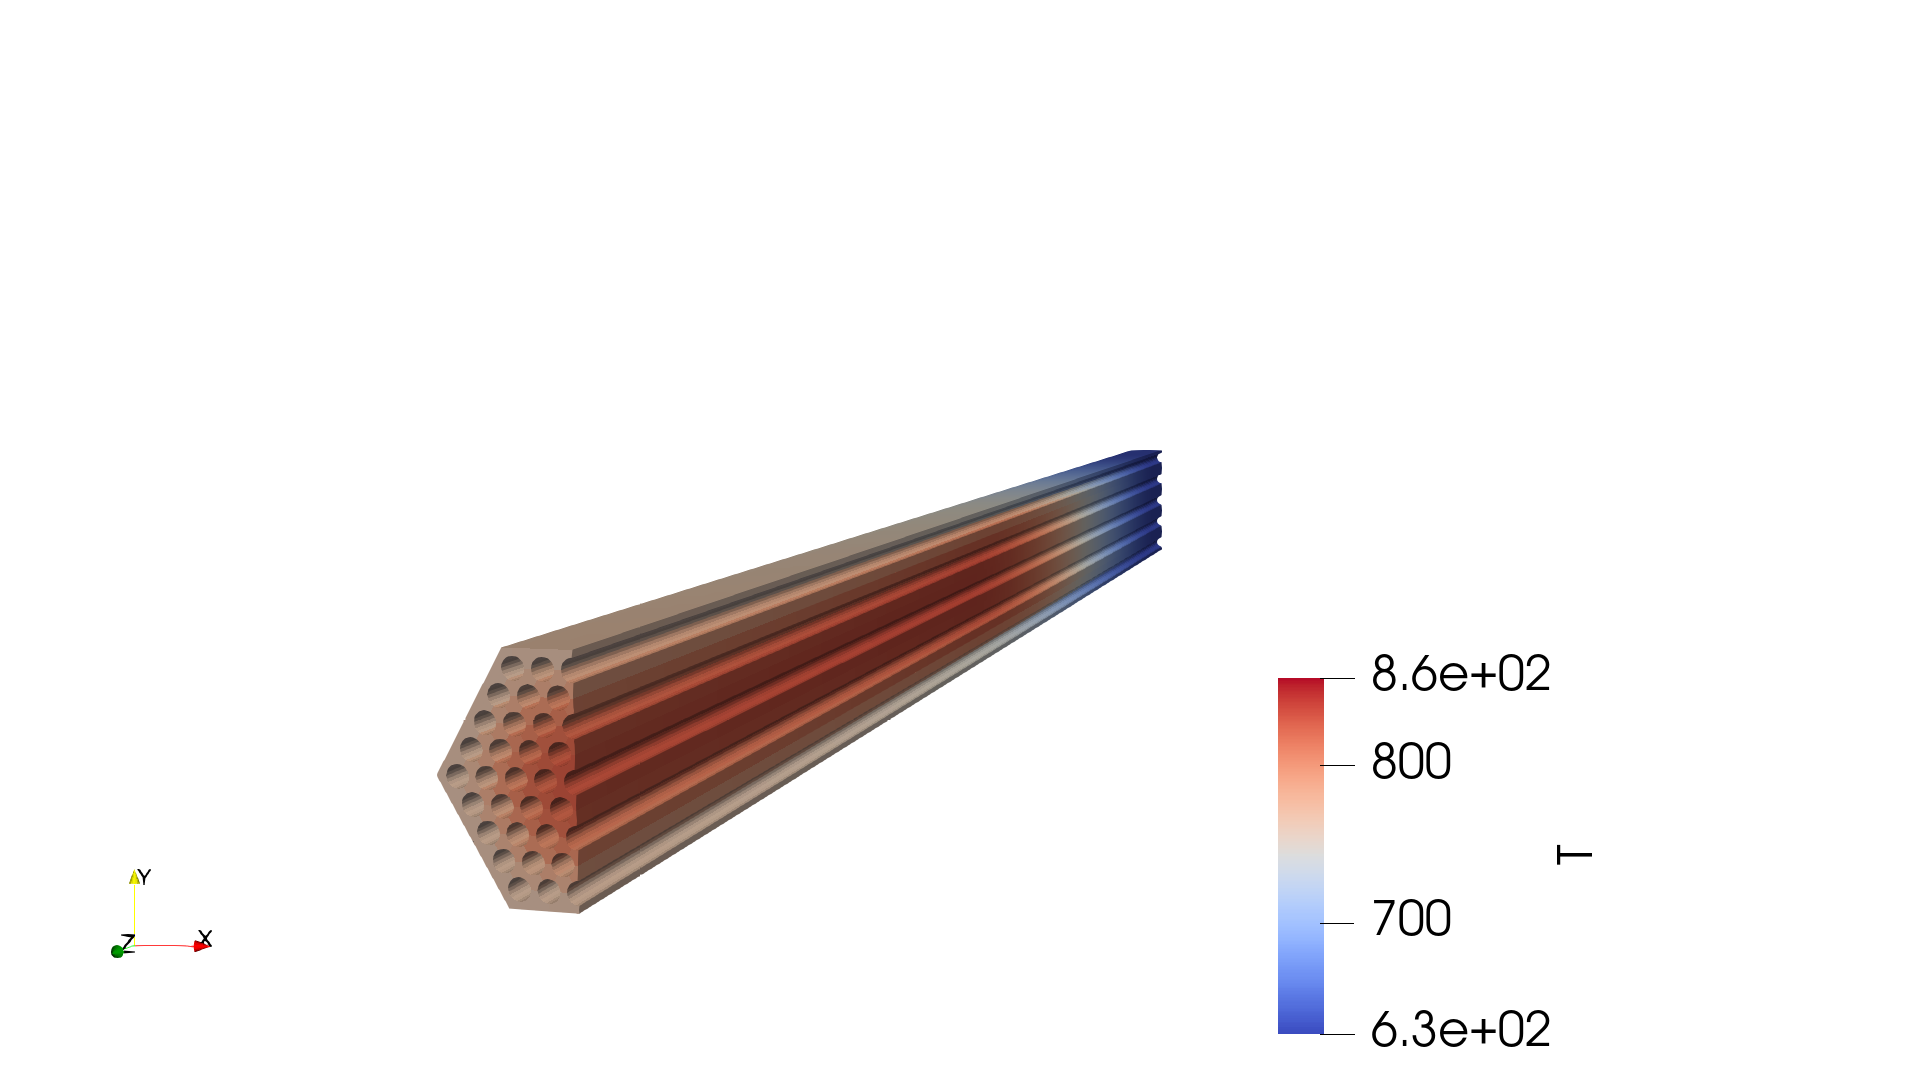
\includegraphics[width=0.70\linewidth]{figures/temperature_field.png}
\caption{Clipped XX09 subchannel temperature field from the present 50-cell MOOSE run.}
\label{fig:temp}
\end{figure}

\section{Independent property basis and engineering checks}

\subsection{Representative sodium properties}
The hand calculations use single representative sodium properties only as engineering checks. For the energy-balance and smooth-pipe pressure-drop estimates, density and heat capacity are evaluated at the mean bulk temperature,
\begin{equation}
T_m=\frac{624.70556+780.651}{2}=\SI{702.68}{K}.
\end{equation}
The Reynolds-number comparison is different: the reported SubChannel assembly Reynolds number is based on an inlet mass-flow-weighted viscosity, so the viscosity check is evaluated at $T_{in}=\SI{624.70556}{K}$ \parencite{moose_subchannel_impl}. These constant values are not substituted into the MOOSE solution; MOOSE evaluates liquid-sodium properties through its fluid-property object \parencite{moose_pbsodium}.

For traceability, the hand-check properties are evaluated from the liquid-sodium correlations documented by SAS4A/SASSYS-1, which are based on established sodium-property correlations including Fink and Leibowitz \parencite{sas_sodium,fink1979}. The density expression is
\begin{equation}
\rho_l=1004.23-0.21390T-1.1046\times10^{-5}T^2,
\end{equation}
which gives $\rho_l(T_m)=\boxed{\SI{848.5}{kg/m^3}}$. The liquid heat-capacity relation is
\begin{equation}
C_l=\frac{A_{28}}{(T_c-T)^2}+\frac{A_{29}}{T_c-T}+A_{30}+A_{31}(T_c-T)+A_{32}(T_c-T)^2,
\end{equation}
with $A_{28}=7.3898\times10^5$, $A_{29}=3.1514\times10^5$, $A_{30}=1.1340\times10^3$, $A_{31}=-2.2153\times10^{-1}$, $A_{32}=1.1156\times10^{-4}$ and $T_c=\SI{2503.3}{K}$ \parencite{sas_sodium}. At $T_m$, this gives $C_l=\SI{1272.06}{J/(kg.K)}$, rounded to \boxed{\SI{1272.2}{J/(kg.K)}} for the notebook calculation.

For viscosity, the SAS4A/SASSYS-1 expression is \parencite{sas_sodium}
\begin{equation}
\mu_l=A_{52}+\frac{A_{53}}{T}+\frac{A_{54}}{T^2}+\frac{A_{55}}{T^3},
\end{equation}
where $A_{52}=3.6522\times10^{-5}$, $A_{53}=0.16626$, $A_{54}=-45.6877$, and $A_{55}=2.8733\times10^4$. Evaluation at the inlet gives
\begin{equation}
\mu_l(T_{in})=\boxed{\SI{3.0345e-4}{Pa.s}}.
\end{equation}

\subsection{Check results}
Applying a steady-flow energy balance with shaft work and kinetic/potential-energy changes neglected gives $T_{out,hand}\approx\SI{780.69}{K}$, compared with \SI{780.651}{K} from MOOSE. The corresponding mass flux is $G=\dot m/A=\SI{2867.8}{kg/(m^2.s)}$. Using the inlet viscosity above,
\begin{equation}
Re=\frac{GD_h}{\mu(T_{in})}\approx2.5886\times10^4,
\end{equation}
which agrees with the MOOSE printout value of 25,886.1 to rounding.

The pressure-drop notebook estimate intentionally uses a much simpler model than the subchannel solver. A smooth-pipe Darcy--Weisbach calculation with the Blasius friction relation $f_D=0.3164Re^{-0.25}$ \parencite{blasius1913} gives approximately \SI{27.0}{kPa} over the \SI{0.612}{m} modeled length when $\rho(T_m)$ is used. The MOOSE pressure-drop postprocessor gives \SI{34.063}{kPa}. The difference is expected because the numerical case applies a wire-wrapped bundle friction treatment rather than a smooth circular-pipe estimate \parencite{moose_ebrii}.

\section{Discretization check and comparison with measurements}

Two additional meshes were run around the 50-cell reference case. The bulk outlet temperature changes by only \SI{0.005}{K} between 50 and 100 cells, while pressure drop changes by about 0.22\%. Local point temperatures respond somewhat more strongly: the largest change among TTC-27--35 between those two meshes is \SI{2.82}{K} (about 0.34\%). These results support use of the 50-cell reference discretization for the comparison, while avoiding a claim of strict mesh independence.

\begin{table}[H]
\centering\small
\caption{Axial discretization study (present calculations).}
\begin{tabular}{@{}rrrr@{}}
\toprule
Axial cells & $T_{out}$ [K] & $\Delta P$ [kPa] & TTC-31 [K] \\
\midrule
25  & 780.653 & 34.034 & 832.898 \\
\textbf{50}  & \textbf{780.651} & \textbf{34.063} & \textbf{831.456} \\
100 & 780.656 & 34.138 & 828.634 \\
\bottomrule
\end{tabular}
\end{table}

The experimental values used for TTC-27 through TTC-35 are taken from the cited ENEA report on EBR-II safety-analysis validation \parencite{delnevo2015}. Figure~\ref{fig:ttc} places those measurements beside the present 50-cell predictions. From the nine paired values, the calculated errors are MAE = \SI{17.47}{K}, RMSE = \SI{19.10}{K}, and MAPE = 2.20\%. The simulation captures the overall thermocouple profile, but the central/hotter locations are mostly high relative to the measurements. TTC-29 has the largest absolute difference (about \SI{29.7}{K}); TTC-34 is predicted below the measured value, so the discrepancy is not a single constant temperature bias.

\begin{figure}[H]
\centering
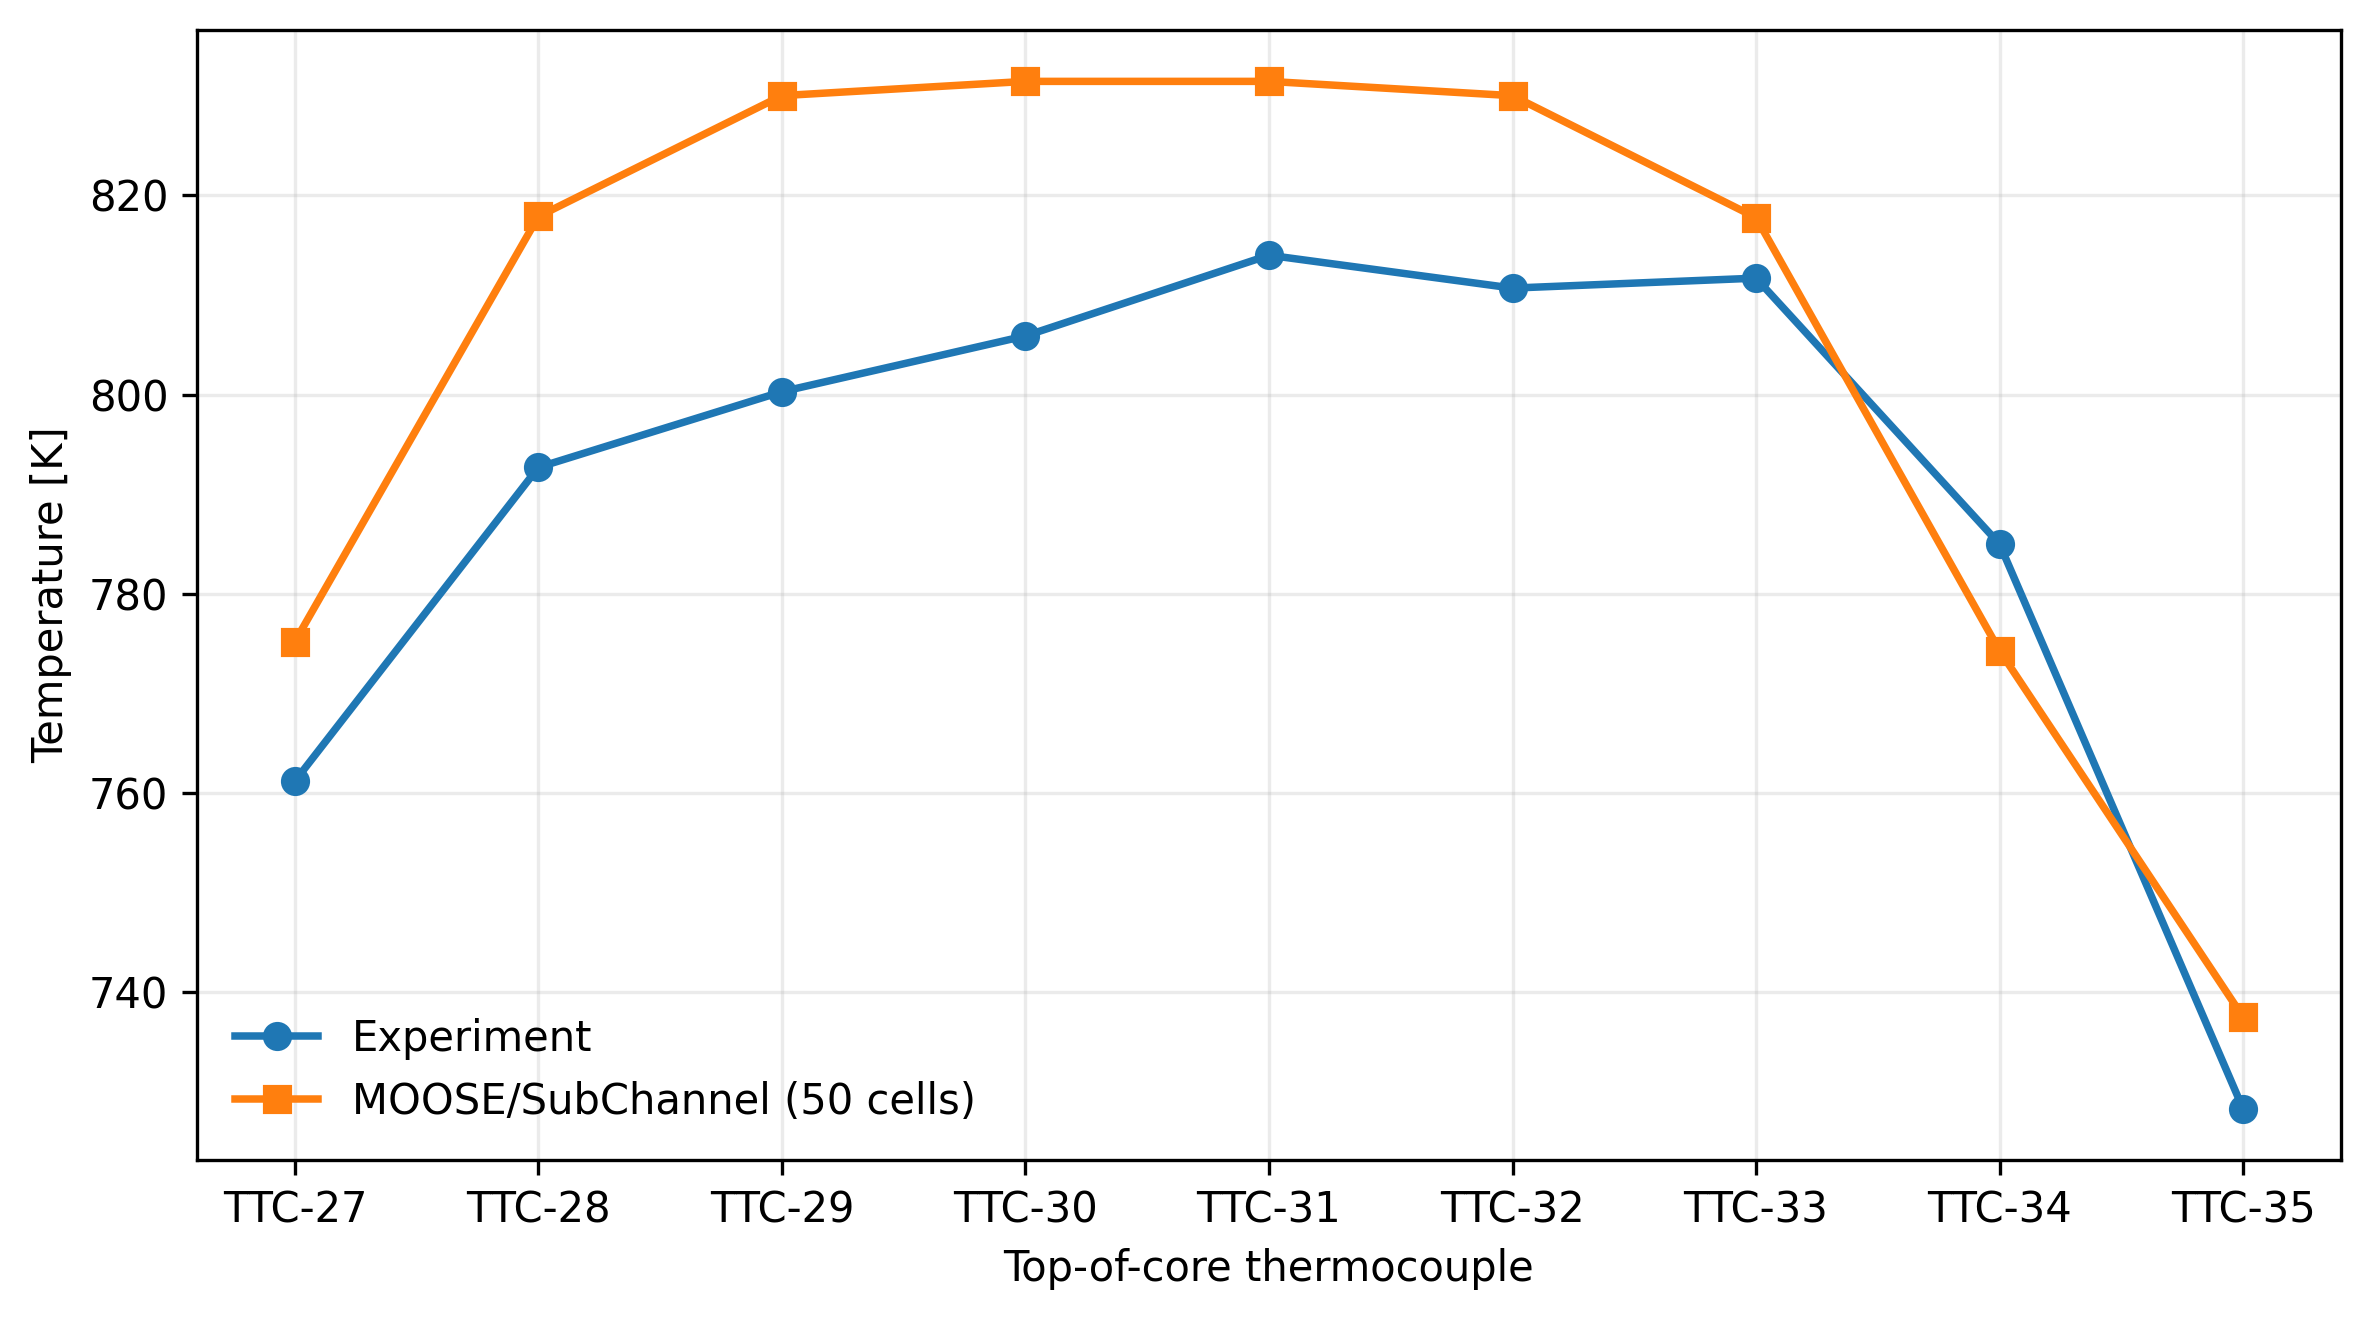
\includegraphics[width=0.80\linewidth]{figures/ttc_validation.png}
\caption{Published SHRT-17 XX09 top-of-core thermocouple measurements \parencite{delnevo2015} and the present 50-cell MOOSE/SubChannel result.}
\label{fig:ttc}
\end{figure}

\section{Conclusions and limits}

The steady XX09 case was reproduced from the cited public MOOSE setup and then subjected to independent checks rather than treated as a black-box result. The bulk energy balance and inlet Reynolds number agree closely with hand calculations; the simple Darcy--Weisbach estimate provides a pressure-drop scale check; and the 25/50/100-cell runs show very small changes in bulk quantities with modestly larger sensitivity at local thermocouple points. Relative to TTC-27--35 measurements, the 50-cell case gives a MAPE of 2.20\%.

The scope remains deliberately narrow: one instrumented subassembly, one pre-transient operating condition, and no claim of full-plant or licensing analysis. Part B is intended to move to the SHRT-17 protected loss-of-flow transient, where the benchmark supplies pump-coastdown and power histories and the physical response evolves toward reduced forced flow and natural circulation \parencite{sumner2012,moose_ebrii}.

\vspace{1mm}
{\small\textbf{Provenance statement.} Argonne provides the experimental benchmark basis \parencite{sumner2012}; the MOOSE project provides the public XX09 validation setup \parencite{moose_ebrii}. The compatibility edit, added pressure-drop output, mesh-variation runs, hand-check calculations, error metrics, plots, and ParaView rendering reported here were produced for this portfolio study. Upstream MOOSE input code is not reproduced in this report; only the postprocessor block added for the present work is shown.}

\printbibliography[title={References}]

\end{document}
